\documentclass{beamer}
\usefonttheme[onlymath]{serif}
\usetheme[numbering=fraction, progressbar=frametitle]{metropolis}
\usepackage{appendixnumberbeamer}
%%% headline section guide
%%% if wish no circles on headline
% \setbeamertemplate{headline}{%
%     \begin{beamercolorbox}[colsep=1.5pt]{upper separation line head}
%     \end{beamercolorbox}
%     \begin{beamercolorbox}{section in head/foot}
%     \vskip2pt\insertsectionnavigationhorizontal{\paperwidth}{}{}\vskip2pt
%         \end{beamercolorbox}%
%         \begin{beamercolorbox}[colsep=1.5pt]{lower separation line head}
%     \end{beamercolorbox}
% }
\usepackage{tikz}
\usetikzlibrary{backgrounds}

\usepackage[utf8]{inputenc}
\usepackage[T1]{fontenc}
\usepackage{textcomp}
\usepackage{amsmath, amssymb, amsthm}

\usepackage[style=authoryear,maxbibnames=9,maxcitenames=2,uniquelist=false,backend=biber,doi=false,url=false]{biblatex}
\renewcommand*{\nameyeardelim}{\addcomma\space} % have comma in parencite
\addbibresource{$BIB} % bibtex location
%%% Small bibliography slide
\setbeamertemplate{bibliography item}[triangle]
\makeatletter
\newcommand{\srcsize}{\@setfontsize{\srcsize}{6.5pt}{6.5pt}}
\makeatother
\renewcommand*{\bibfont}{\srcsize}

\usepackage{import}
\usepackage{pdfpages}
\usepackage{transparent}
\usepackage{xcolor}

\newcommand{\blue}[1]{\textcolor{blue}{#1}}
\newcommand{\red}[1]{\textcolor{red}{#1}}
\newcommand{\orange}[1]{\textcolor{orange}{#1}}

\graphicspath{ {./figures} }
\newcommand{\inkfig}[2][1]{%
    \def\svgwidth{#1\columnwidth}
    \import{./figures/}{#2.pdf_tex}
}

%%%%%% Template
\usepackage{hyperref}
\definecolor{links}{HTML}{2A1B81}

%% beaver (red) style:
% \usecolortheme{beaver}
% \setbeamercolor{block body}{bg=gray!30!white}
% \setbeamercolor{block title}{bg=darkred!70, fg=black!2}
% \hypersetup{colorlinks=true,allcolors=red}

%% seahorse style:
\usecolortheme{seahorse}
\setbeamercolor{block body}{bg=mDarkTeal!30}
\setbeamercolor{block title}{bg=mDarkTeal,fg=black!2}
\hypersetup{colorlinks=true,allcolors=links}
%%%%%% Template

\pdfsuppresswarningpagegroup=1

\title{Unit 9 Quiz Supplement: shift in wage-setting curve}
\author{Hui-Jun Chen}
\institute{The Ohio State University}
\date{\today}

\begin{document}

\maketitle

% \frame{%
%    \maketitle
%    \begin{center}
%        \includegraphics
%			[width=0.2\textwidth]
%			{./figures/Ohio_State_University_seal}
%    \end{center}
% }

\begin{frame}{Recap: labor-discipline model}
\label{slide:Recap__labor_discipline_model}
    [Page 31 in Unit 9 slide] What shifts the best response curve of workers?
    \begin{itemize}
        \item the utility of the things that the wage can buy
        \item the disutility of effort
        \item the reservation wage
        \item the probability of getting fired at each effort level
    \end{itemize}
    $ \Rightarrow  $ \red{NO one-to-one relationship between best response curve and unemployment rate}
\end{frame}

\begin{frame}{First confusing concept: Shift of best-response curve}
\label{First_confusing_concept__Shift_of_best_response_curve}
    Both ``better'' and ``worse'' is for \blue{individual} workers, which means both best response curve below can represent the \textbf{same} level of unemployment.

    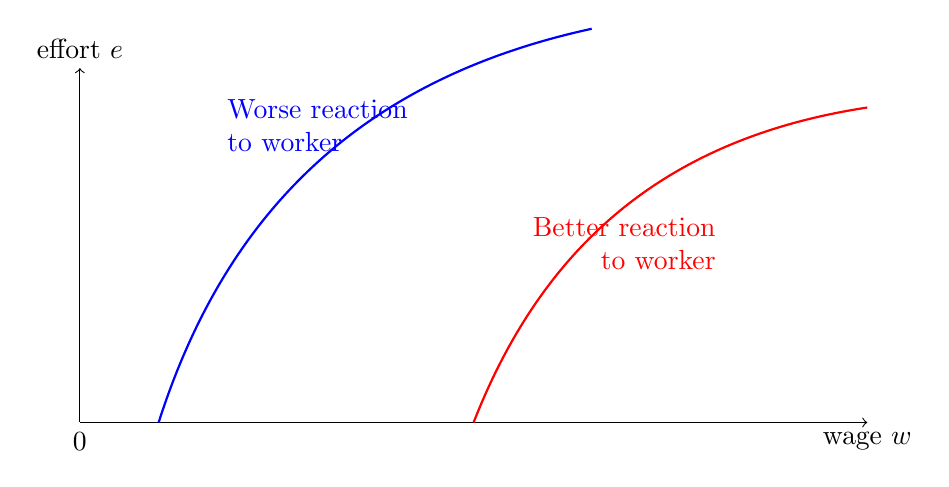
\begin{tikzpicture}
        \pgfmathsetmacro{\x}{10}
        \pgfmathsetmacro{\y}{4}
        % \draw[very thin,color=gray] (0,0) grid (\x, \y); % gray grid
        \draw[->] (0,0) node[below]{ $ 0 $  } -- (\x,0) node[below]{wage $w$};   % label x axis
        \draw[->] (0,0) -- (0,\y + 0.5) node[above]{effort $e$};   % label y axis
        \draw[thick, blue]
            (1, 0) to[bend left]
            node[align=left, above]{Worse reaction\\to worker}
            (6.5, 5);
        \draw[thick, red]
            (5, 0) to[bend left]
            node[align=right, below]{Better reaction\\to worker}
            (10, 4);
    \end{tikzpicture}

\end{frame}

\begin{frame}{Recap: Derivation of wage-setting curve}
\label{slide:Recap__Derivation_of_wage_setting_curve}
    IF now the shift of best-response curve is driven by change in unemployment, we can depict the \textbf{relationship between wage and unemployment}, and thus derive the wage-setting curve in the whole economy.

    The figure below \textbf{switches the $ x $-axis and $ y $-axis} so that both the figure from labor-discipline model and wage-setting curve can be directly linked.

\end{frame}


\begin{frame}
    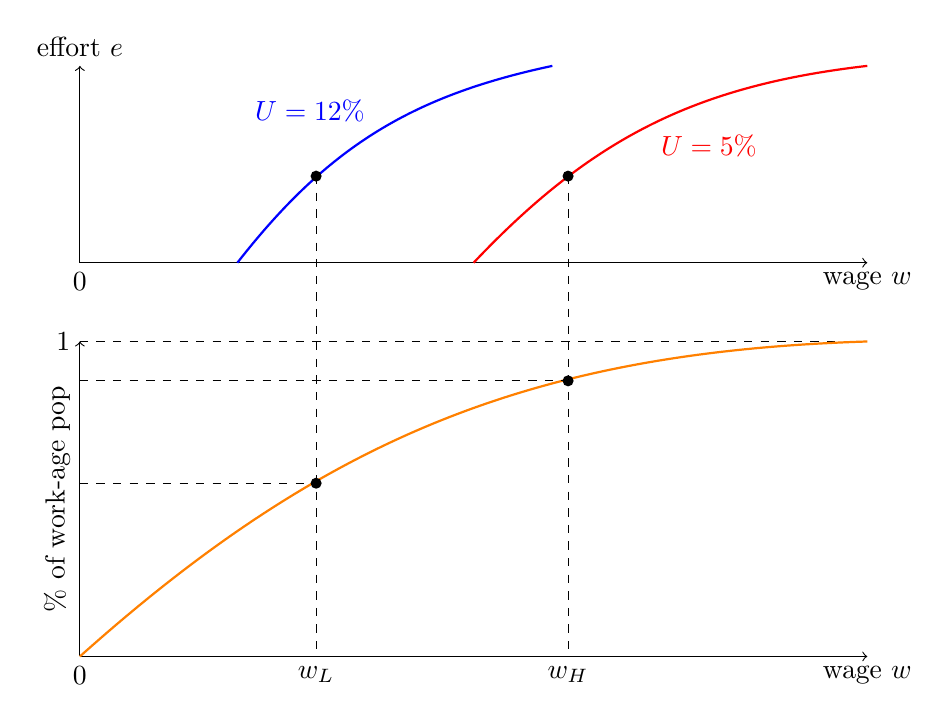
\begin{tikzpicture}
        \pgfmathsetmacro{\x}{10}
        \pgfmathsetmacro{\y}{7}
        % \draw[very thin,color=gray] (0,0) grid (\x, \y); % gray grid
        \draw[->] (0, 5) node[below]{ $ 0 $  } -- (\x,5) node[below]{wage $w$};   % label x axis
        \draw[->] (0, 5) -- (0, \y + 0.5) node[above]{effort $e$};   % label y axis
        \draw[thick, blue] (2, 5) to[bend left=20] node[above left]{$U=12\%$} (6,\y+0.5);
        \fill (3, 6.1) circle (2pt);
        \draw[thick, red] (5, 5) to[bend left=20] node[below right]{$U=5\%$} (10,\y+0.5);
        \fill (6.2, 6.1) circle (2pt);
        \draw[->] (0, 0) node[below]{ $ 0 $  } -- (\x,0) node[below]{wage $w$} ;   % label x axis
        \draw[->] (0, 0) -- node[above, rotate=90]{\% of work-age pop} (0, \y/2 + 0.5) ;   % label y axis
        \draw[dashed]  (0, \y/2+0.5) node[left]{$1$} -- (\x, \y/2+0.5);
        \draw[thick, orange] (0, 0) to[bend left=20] (10,\y/2+0.5);
        \fill (3, 2.2) circle (2pt);
        \fill (6.2, 3.5) circle (2pt);
        \draw[dashed] (0, 2.2) -- (3, 2.2);
        \draw[dashed] (0, 3.5) -- (6.2, 3.5);
        \draw[dashed] (3, 6.1) -- (3, 0) node[below]{$w_L$};
        \draw[dashed] (6.2, 6.1) -- (6.2, 0) node[below]{$w_H$};
    \end{tikzpicture}
\end{frame}

\begin{frame}{Second confusing concept: Shift of wage-setting curve}
\label{slide:Second_confusing_concept__Shift_of_wage_setting_curve}
    Even though wage-setting curve is derived by IMPOSING the change of best-response curve is because of change in unemployment, yet as I mentioned before, \textbf{other factors} can also shift the best-response curve, and \textbf{change in any factors other than (un)employment and wage will also shift the wage-setting curve}.

    Assume the shift in curves within the figure in next slide is originated from \textit{more generous unemployment insurance scheme}, which is NOT related to unemployment rate.

    $ \Rightarrow  $ higher unemployment benefit$ \Rightarrow  $ workers better off $ \Rightarrow  $ best response curve shift \textbf{rightward/downward} $ \Rightarrow  $ equilibrium wage is \textbf{higher} $ \Rightarrow  $ wage curve shift \textbf{rightward/downward}.

\end{frame}

\begin{frame}
    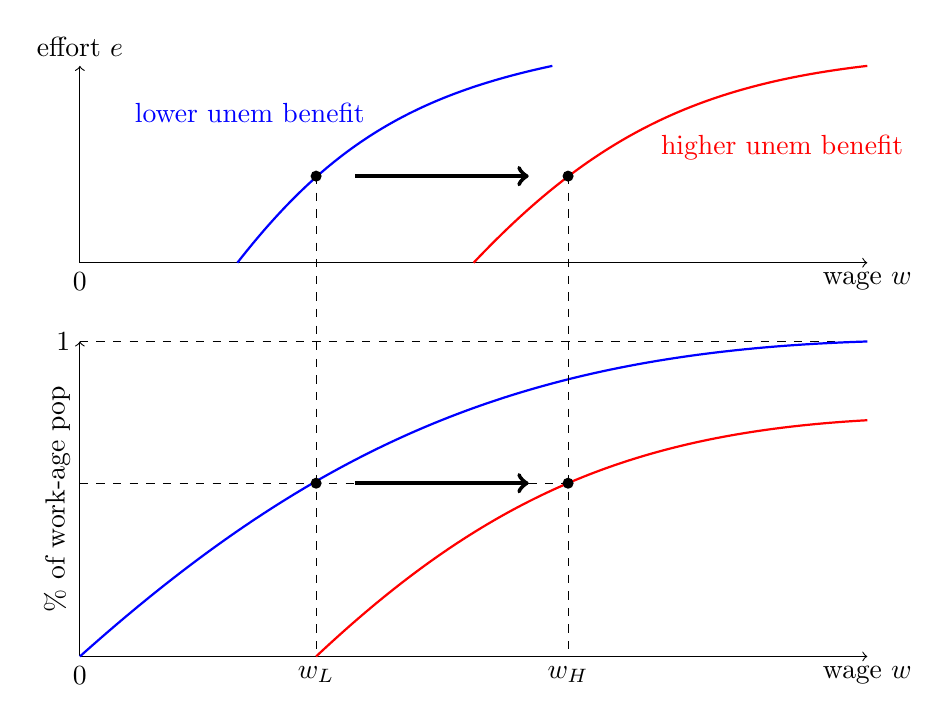
\begin{tikzpicture}
        \pgfmathsetmacro{\x}{10}
        \pgfmathsetmacro{\y}{7}
        % \draw[very thin,color=gray] (0,0) grid (\x, \y); % gray grid
        \draw[->] (0, 5) node[below]{ $ 0 $  } -- (\x,5) node[below]{wage $w$};   % label x axis
        \draw[->] (0, 5) -- (0, \y + 0.5) node[above]{effort $e$};   % label y axis
        \draw[thick, blue] (2, 5) to[bend left=20] node[above left]{lower unem benefit} (6,\y+0.5);
        \fill (3, 6.1) circle (2pt);
        \draw[thick, red] (5, 5) to[bend left=20] node[below right]{higher unem benefit} (10,\y+0.5);
        \fill (6.2, 6.1) circle (2pt);
        \draw[ultra thick, ->] (3 + 0.5, 6.1) -- (6.2 - 0.5, 6.1);
        \draw[->] (0, 0) node[below]{ $ 0 $  } -- (\x,0) node[below]{wage $w$} ;   % label x axis
        \draw[->] (0, 0) -- node[above, rotate=90]{\% of work-age pop} (0, \y/2 + 0.5) ;   % label y axis
        \draw[dashed]  (0, \y/2+0.5) node[left]{$1$} -- (\x, \y/2+0.5);
        \draw[thick, blue] (0, 0) to[bend left=20] (10,\y/2+0.5);
        \draw[thick, red] (3, 0) to[bend left=20] (10,\y/2-0.5);
        \fill (3, 2.2) circle (2pt);
        \fill (6.2, 2.2) circle (2pt);
        \draw[ultra thick, ->] (3 + 0.5, 2.2) -- (6.2 - 0.5, 2.2);
        \draw[dashed] (0, 2.2) -- (6.2, 2.2);
        \draw[dashed] (3, 6.1) -- (3, 0) node[below]{$w_L$};
        \draw[dashed] (6.2, 6.1) -- (6.2, 0) node[below]{$w_H$};
    \end{tikzpicture}
\end{frame}

\begin{frame}{Correction of confusion: Flip the figure back!}
\label{slide:Correction_of_confusion__Flip_the_figure_back_}
    Before: shift \textbf{rightward/downward} is better for workers.

    Now: shift to the \textbf{leftward/upward} is better for workers.

    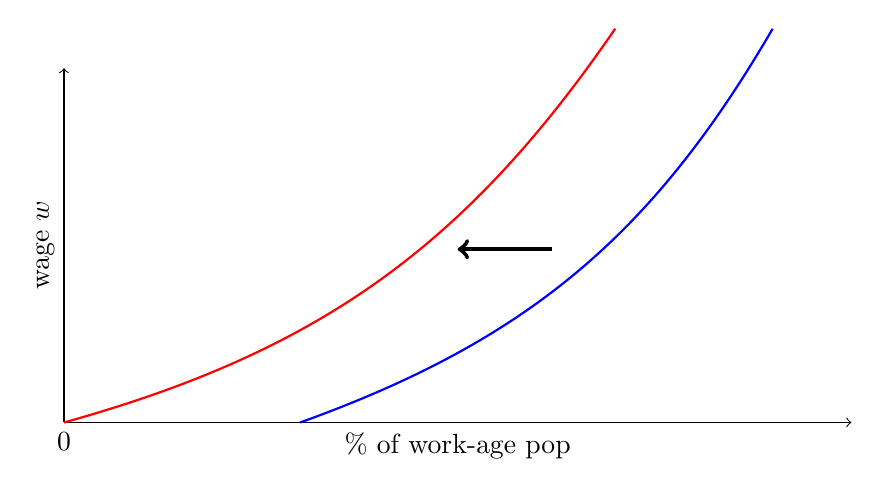
\begin{tikzpicture}
        \pgfmathsetmacro{\x}{10}
        \pgfmathsetmacro{\y}{4}
        % \draw[very thin,color=gray] (0,0) grid (\x, \y); % gray grid
        \draw[->] (0,0) node[below]{ $ 0 $  } -- node[below]{\% of work-age pop} (\x,0);   % label x axis
        \draw[->] (0,0) -- node[above, rotate=90]{wage $w$} (0,\y + 0.5) ;   % label y axis
        \draw[ultra thick, ->] (6.2, 2.2) -- (5, 2.2);
        \draw[thick, red] (0, 0) to[bend right=20] (7, 5);
        \draw[thick, blue] (3, 0) to[bend right=20] (9, 5);
    \end{tikzpicture}

\end{frame}

\end{document}

